
\documentclass[11pt]{beamer}
\usepackage{booktabs}
\usepackage{array}
\usepackage{eulervm}
\usepackage{tcolorbox}

\newcommand{\sgap}{\vspace{0.5em}}
\newcommand{\bgap}{\vspace{0.8em}}

% Fonts --------------------------------------------------------------------------

\usepackage[scaled]{helvet}
\usepackage[T1]{fontenc}

% If using XeLaTeX:
% \usepackage{fontspec}
% \setmonofont[Path=./fonts/,Scale=0.9]{JetBrainsMono.ttf}
% \setmainfont[Path=./fonts/]{KingsBureauGrot-FiveOne.ttf}
% \setsansfont[Path=./fonts/]{KingsCaslon.ttf}
% \setbeamerfont{title page}{family=\rmfamily}
% \setbeamerfont{frametitle}{family=\rmfamily}

% References ------------------------------------------------------------------

\usepackage[%
  backend     = bibtex,
  style       = numeric,
  sorting     = ynt,
  sortcites   = true,
  autocite    = superscript
]{biblatex}

\addbibresource{references.bib}

% tcolorbox -------------------------------------------------------------------

\newtcolorbox{cbox}[3][]
{
  colframe = #2!5,
  colback  = #2!5,
  coltitle = #2!50!black,  
  colbacktitle = #2!5,
  lefttitle = 1mm,
  toptitle = 2mm,
  bottomtitle = 0mm,
  colupper = #2!50!black,  
  title    = {#3},
  fonttitle = \bfseries\large,
  #1,
  arc=0.5mm,
  left=2.5mm,
  before upper={\setbeamercolor{item}{fg=#2!50!black}},
  after upper={\setbeamercolor{item}{fg=#2!50!black}}
}

\makeatletter
\def\beamer@origitem{%
  \@inmatherr\item\@ifnextchar[\@item{\@noitemargtrue\@item[\@itemlabel]%
  \csname beamer@thcfg@\beameritemnestingprefix item\endcsname% Insert colour in \beamer@thc@fg
  \ifx\beamer@thc@fg\@empty\relax\else\color{\beamer@thc@fg}\fi% Execute colour
  }}
\makeatother

\usepackage{graphicx}
\newcommand*{\img}[1]{%
    \raisebox{-.3\baselineskip}{%
        \includegraphics[
        height=\baselineskip,
        width=\baselineskip,
        keepaspectratio,
        ]{#1}%
    }%
}

\title[The \texttt{pmsims} package for R]{
    A simulation approach to calculating minimum sample sizes for prediction
    modelling
}
\subtitle{The \texttt{pmsims} package for R}
\date{29$^{\text{th}}$ August 2023}
\author[Biostatistics \& Health Informatics, KCL]{%
	Ewan Carr, Gordon Forbes, Diana Shamsutdinova, Daniel Stahl,
	and Felix Zimmer}
\institute[]{Department of Biostatistics \& Health Informatics\\ King's College London}
\titlegraphic{
\includegraphics[height=1.5cm]{figures/kcl.png}}
\setbeamertemplate{navigation symbols}{}
\setbeamertemplate{footline}[frame number]

% Theme
\definecolor{KCLpurple}{RGB}{80, 20, 145}
\definecolor{KCLred}{RGB}{226, 35, 26}
\definecolor{KCLhotpink}{RGB}{200, 50, 150}
\definecolor{KCLpurple}{RGB}{80, 20, 145}
\definecolor{KCLseablue}{RGB}{0, 90, 210}
\definecolor{KCLtealblue}{RGB}{0, 154, 166}
\definecolor{KCLpeagreen}{RGB}{0, 181, 136}
\definecolor{KCLpantone}{RGB}{0, 35, 149}
\usecolortheme[named=KCLseablue]{structure}
\setbeamercolor{alerted text}{fg=KCLhotpink}

\setbeamertemplate{itemize items}[circle]
\setbeamertemplate{enumerate items}[default]

\newenvironment{itemize*}%
{\begin{itemize}%
		\setlength{\itemsep}{100pt}%
		\setlength{\parskip}{0pt}}%
		{\end{itemize}}

\begin{document}

\maketitle

\section{Introduction}

\begin{frame}[c]{30-second version}
	\Large
	\begin{enumerate}
		\setlength{\itemsep}{12pt}

		\item Most prediction models use small samples.

		\item Small samples cause overfitting and imprecise estimates.

		\item Existing tools can estimate minimum samples for continuous,
		      binary, and survival outcomes.

		\item Nothing exists for other models or data types.

	\end{enumerate}

	\sgap

	\begin{cbox}{KCLtealblue}{}
		We're developing a simulation-based approach that works with any
		outcome or method.
	\end{cbox}
	\vspace{-1em}
\end{frame}

\begin{frame}[c]
	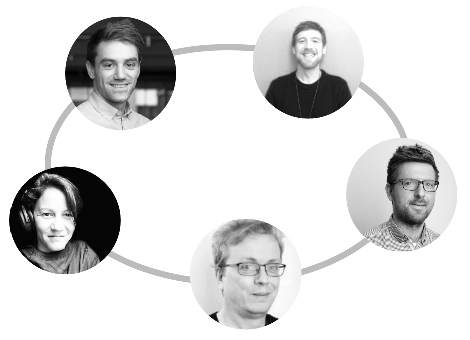
\includegraphics[width=\textwidth]{figures/group_photos.pdf}
\end{frame}

\begin{frame}[t]{This talk}
	\large
	\begin{enumerate}
		\item Background
		      \begin{itemize}
			      \item What's the problem we're trying to solve?
			      \item What solutions currently exist?
		      \end{itemize}
		\item Our simulation-based approach
		      \begin{itemize}
			      \item Workflow and user interface
			      \item How it compares to other packages
		      \end{itemize}
		\item Demonstration
		\item Development status and next steps
	\end{enumerate}

	\bgap
\end{frame}

\begin{frame}[c]
	\centering
	\begin{columns}
		\begin{column}[c]{0.6\textwidth}
			We're still developing the package.

			Your feedback is welcome.

			Please get in touch.
		\end{column}
		\begin{column}[c]{0.3\textwidth}
			\centering
			
\includegraphics[width=\linewidth]{figures/roadwork-sign.png}
		\end{column}
	\end{columns}

\end{frame}

\section{Background}

\begin{frame}[t]{What's the problem?}

	% Say: Prediction models can inform treatment decisions, facilitate
	% screening, and enable stratified care.

	Hundreds of prediction models are developed each year. Most have
	inadequate samples.

	\begin{cbox}{KCLseablue}{}
		\large
		\begin{itemize}
			\item Insufficient sample sizes was the most common cause of bias
			      in 731 models for COVID-19.\autocite{wynants2020}
			\item Inadequate samples were found in: \vspace{0.5em}
		\end{itemize}
		\begin{tabular}{lp{.8\textwidth}}
			{\Huge \alert{67\%}} & models for COVID-19\autocite{wynants2020}                      \\[0.5em]
			{\Huge \alert{56\%}} & models using supervised machine learning\autocite{navarro2021} \\[0.5em]
			{\Huge \alert{73\%}} & models in psychiatry\autocite{meehan2022}                      \\[0.3em]
		\end{tabular}
		\begin{itemize}
			\item Just \alert{8\%} of machine learning models in oncology
			      reported a sample size justification\autocite{dhiman2022}.
		\end{itemize}
	\end{cbox}
\end{frame}

\begin{frame}[t]{Inadequate samples = research waste}

	\begin{itemize}
		\item Inadequate samples lead to overfitting and inaccurate estimates
		      of model parameters.

		      % Overfitting is where the model captures idiosyncrasies
		      % of the development sample, producing inflated estimates of predictive
		      % performance that cannot be replicated in the target population.

		\item This may generate inappropriate decisions about patient care or
		      lead to models not being implemented into clinical practice.

		\item Data collection can be invasive and inconvenient and diverts
		      resources from other activities that benefit patients.

	\end{itemize}

	\begin{cbox}{KCLpurple}{}
		\large
		Ensuring sample sizes are sufficient \textbf{before model development}
		would improve patient outcomes by avoiding models developed with
		inadequate samples and reducing participant burden.
	\end{cbox}

\end{frame}

\begin{frame}[t]{What tools currently exist?}

	\centering
	\begin{columns}
		\begin{column}[c]{0.6\textwidth}
			\centering
			Most studies ignore sample size.
		\end{column}
		\begin{column}[c]{0.35\textwidth}
			
\includegraphics[width=\textwidth]{figures/bury-head.png}
		\end{column}
	\end{columns}

	\vspace{3em}

	Or use rules of thumb (e.g., 10 events per variable) that have no
	rationale in prediction modelling\autocite{vansmeden2016}.

	% However, this rule of thumb has been shown to have no rationale, especially
	% in prediction model research, as its evidence base is mainly informed by
	% simulation studies that investigate the performance of estimating
	% covariate-outcome relationships.
	% https://bmcmedresmethodol.biomedcentral.com/articles/10.1186/s12874-023-02008-1

	\vspace{3em}
	In 2018, Riley et al released \texttt{pmsampsize} for R and Stata.

\end{frame}

\begin{frame}[t]{\texttt{pmsampsize}}
	\begin{columns}
		\begin{column}[c]{0.5\textwidth}

		\end{column}
		\begin{column}[c]{0.5\textwidth}
			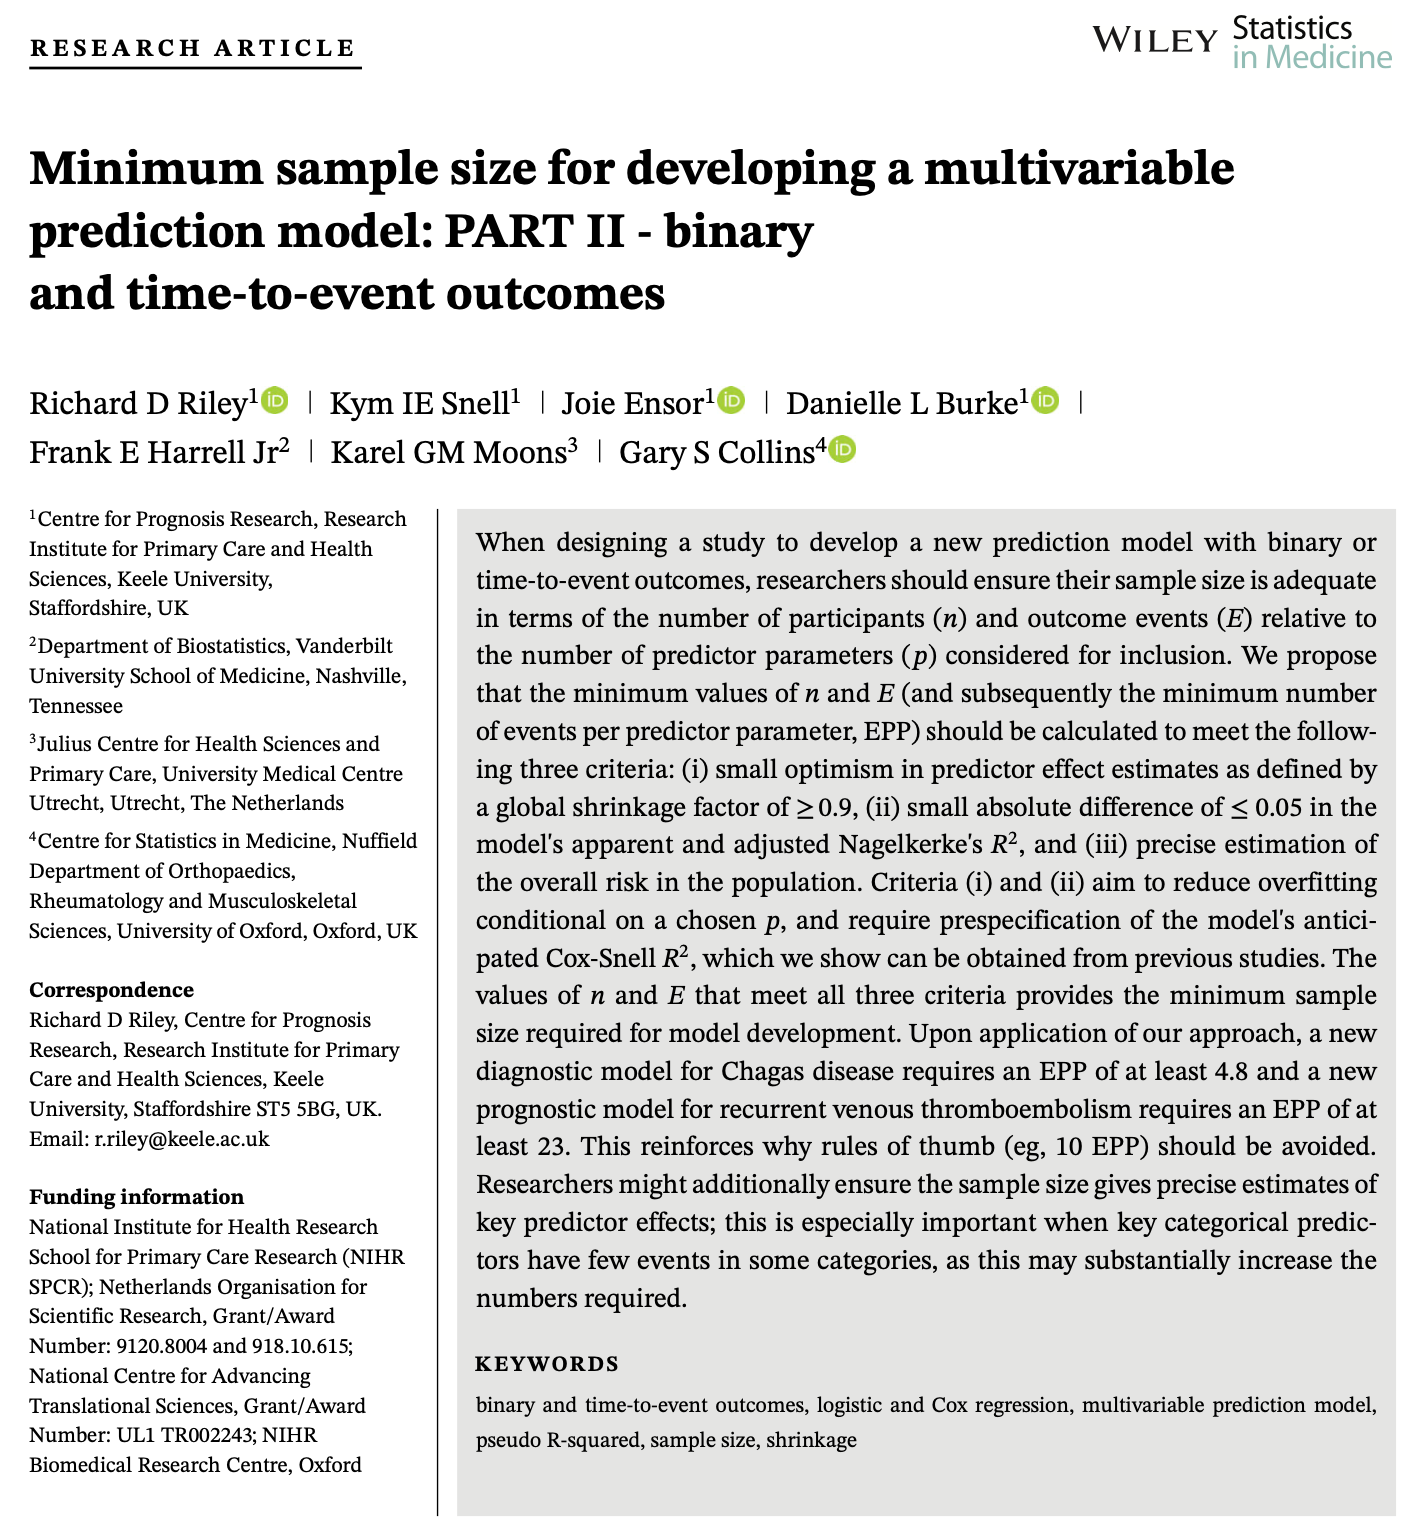
\includegraphics[width=\textwidth]{figures/riley2.png}

		\end{column}
	\end{columns}

	pmsampsize has methods for simple continuous, binary, and survival
	outcome.

\end{frame}

\begin{frame}{pmsampsize}

	The package identifies the minimum sample that results in: \\[1em]

	\centering

	\begin{tabular}{l>{\raggedright\arraybackslash}p{12em}>{\raggedright\arraybackslash}p{12em}}
		           & \textbf{Continuous}                                          & \textbf{Binary} \\ \midrule
		i.         & \multicolumn{2}{p{24em}}{Small optimism in predictor effect
		estimates, indicated by a global shrinkage factor of ≥ 0.9.}                                \\ \midrule
		ii.        & \multicolumn{2}{p{20em}}{Small absolute difference of ≤ 0.05
		in the apparent and adjusted $R^2$}                                                         \\ \midrule
		iii.       & Precise estimation of the model's residual standard
		deviation. & Precise estimation of the overall risk in the
		population.                                                                                 \\ \midrule
		iv.        & Precise estimation of the model intercept.                   &                 \\
	\end{tabular}

\end{frame}

\begin{frame}[c]{We \img{figures/heart.png} pmsampsize, but\ldots}
	\large

	We increasingly need to estimate minimum samples for:

	\begin{cbox}{KCLtealblue}{Other models}
		\begin{itemize}
			\item Regularised regression (e.g., LASSO, elastic net)
			\item Machine learning algorithms (e.g., random forests, gradient
			      boosting)
		\end{itemize}
	\end{cbox}

	\begin{cbox}{KCLhotpink}{Other types of data}{}
		\begin{itemize}
			\item Longitudinal and repeated measures
			\item Clustered data
		\end{itemize}
	\end{cbox}

	We're creating a simulation-based framework to estimate sample sizes
	for prediction.

\end{frame}

\begin{frame}[t]{The \alert{pmsims} package for R}

    Key features:

	\begin{itemize}
		\item Able to estimate minimum sample sizes for \alert{any model or data
		      type};
		\item Provides defaults for common model and data types;
		\item Efficient estimation.
	\end{itemize}

    This last point is key:\ most machine learning approaches are too
    computationally demanding for conventional simulation approaches.

\end{frame}

\begin{frame}[t]{Our approach}

	\begin{cbox}{KCLpeagreen}{Setting}
		\begin{enumerate}
			\setlength{\itemsep}{7pt}
			\item A study population represented by outcome-related individual
			      characteristics (i.e., candidate predictors).
			\item A chosen statistical or machine learning model.
			\item Expected achievable performance (e.g., $R^2$, AUC) without
			      sample size constraints, $P^{*}$.
			\item Minimum acceptable performance of the model, $P^{OK}$.
		\end{enumerate}
	\end{cbox}

    \onslide<2>
	\sgap
    \centering
	
\includegraphics[height=3.6em]{figures/target.pdf}
    \hspace{0.7em}
    \large
	\parbox[b]{0.8\textwidth}{
        \raggedright
        \textcolor{KCLpantone}{ Find the minimum sample
	    that ensures test performance of $P^{OK}$ with probability of 80\%,
	    given the population, predictors, and $P^{*}$. } }

	% i.e., drawing a random sample of size $n$ will result in a model with
	% performance $>P^{OK}$ in more than 80\% of cases.

\end{frame}

\begin{frame}[c,fragile]{How does it work?}

    \begin{columns}
        \begin{column}[c]{0.5\textwidth}
            \centering
            \only<1>{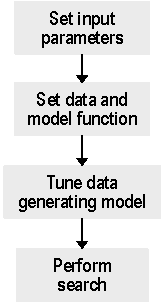
\includegraphics[width=0.7\textwidth]{figures/workflow-a.pdf}}
            \only<2>{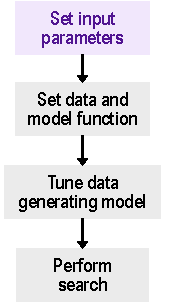
\includegraphics[width=0.7\textwidth]{figures/workflow-b.pdf}}
            \only<3>{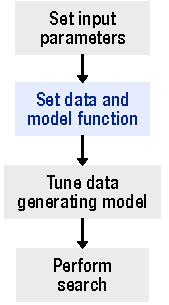
\includegraphics[width=0.7\textwidth]{figures/workflow-c.pdf}}
            \only<4>{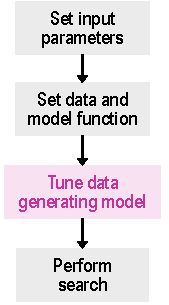
\includegraphics[width=0.7\textwidth]{figures/workflow-d.pdf}}
            \only<5>{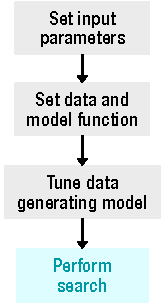
\includegraphics[width=0.7\textwidth]{figures/workflow-e.pdf}}
        \end{column}
        \begin{column}[c]{0.5\textwidth}
            Some text here.
    
        \end{column}
    \end{columns}

\end{frame}

\begin{frame}[t]{Maybe put slide here about conceptual differences vs.\ pmsampsize?}

\end{frame}

\begin{frame}[c]{Our approach}

	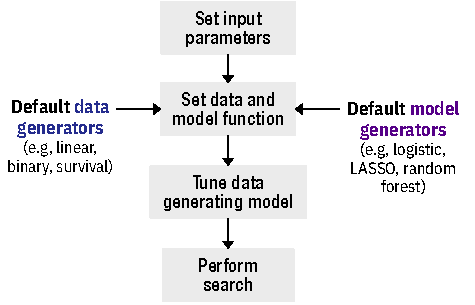
\includegraphics[width=\textwidth]{figures/workflow1.pdf}

\end{frame}

\begin{frame}[t]{Slide explaining input parameters}

	\begin{itemize}
		\item \texttt{simulate\_continuous}
		\item \texttt{simulate\_binary}
		\item \texttt{simulate\_survival}
	\end{itemize}

	Which each call:

	\begin{itemize}
		\item \texttt{simulate\_custom}
	\end{itemize}

\end{frame}

\begin{frame}[t]{Slide explaining default data and model generators}

	List default data/model/metrics.

\end{frame}

\begin{frame}{Performing the search:\ \texttt{mlpwr}}

	\begin{cbox}{KCLpurple}{}
		A simulation-based approach with complex data or models would be too
		slow.
	\end{cbox}

	\begin{columns}
		\begin{column}[c]{0.5\textwidth}
			\texttt{mlpwr} is a R package by Felix Zimmer and Rudolf Debelak at
			the University of Zurich.
			\begin{quote}
				``A Power Analysis Toolbox to Find Cost-Efficient Study Designs''
			\end{quote}
		\end{column}
		\begin{column}[c]{0.5\textwidth}
			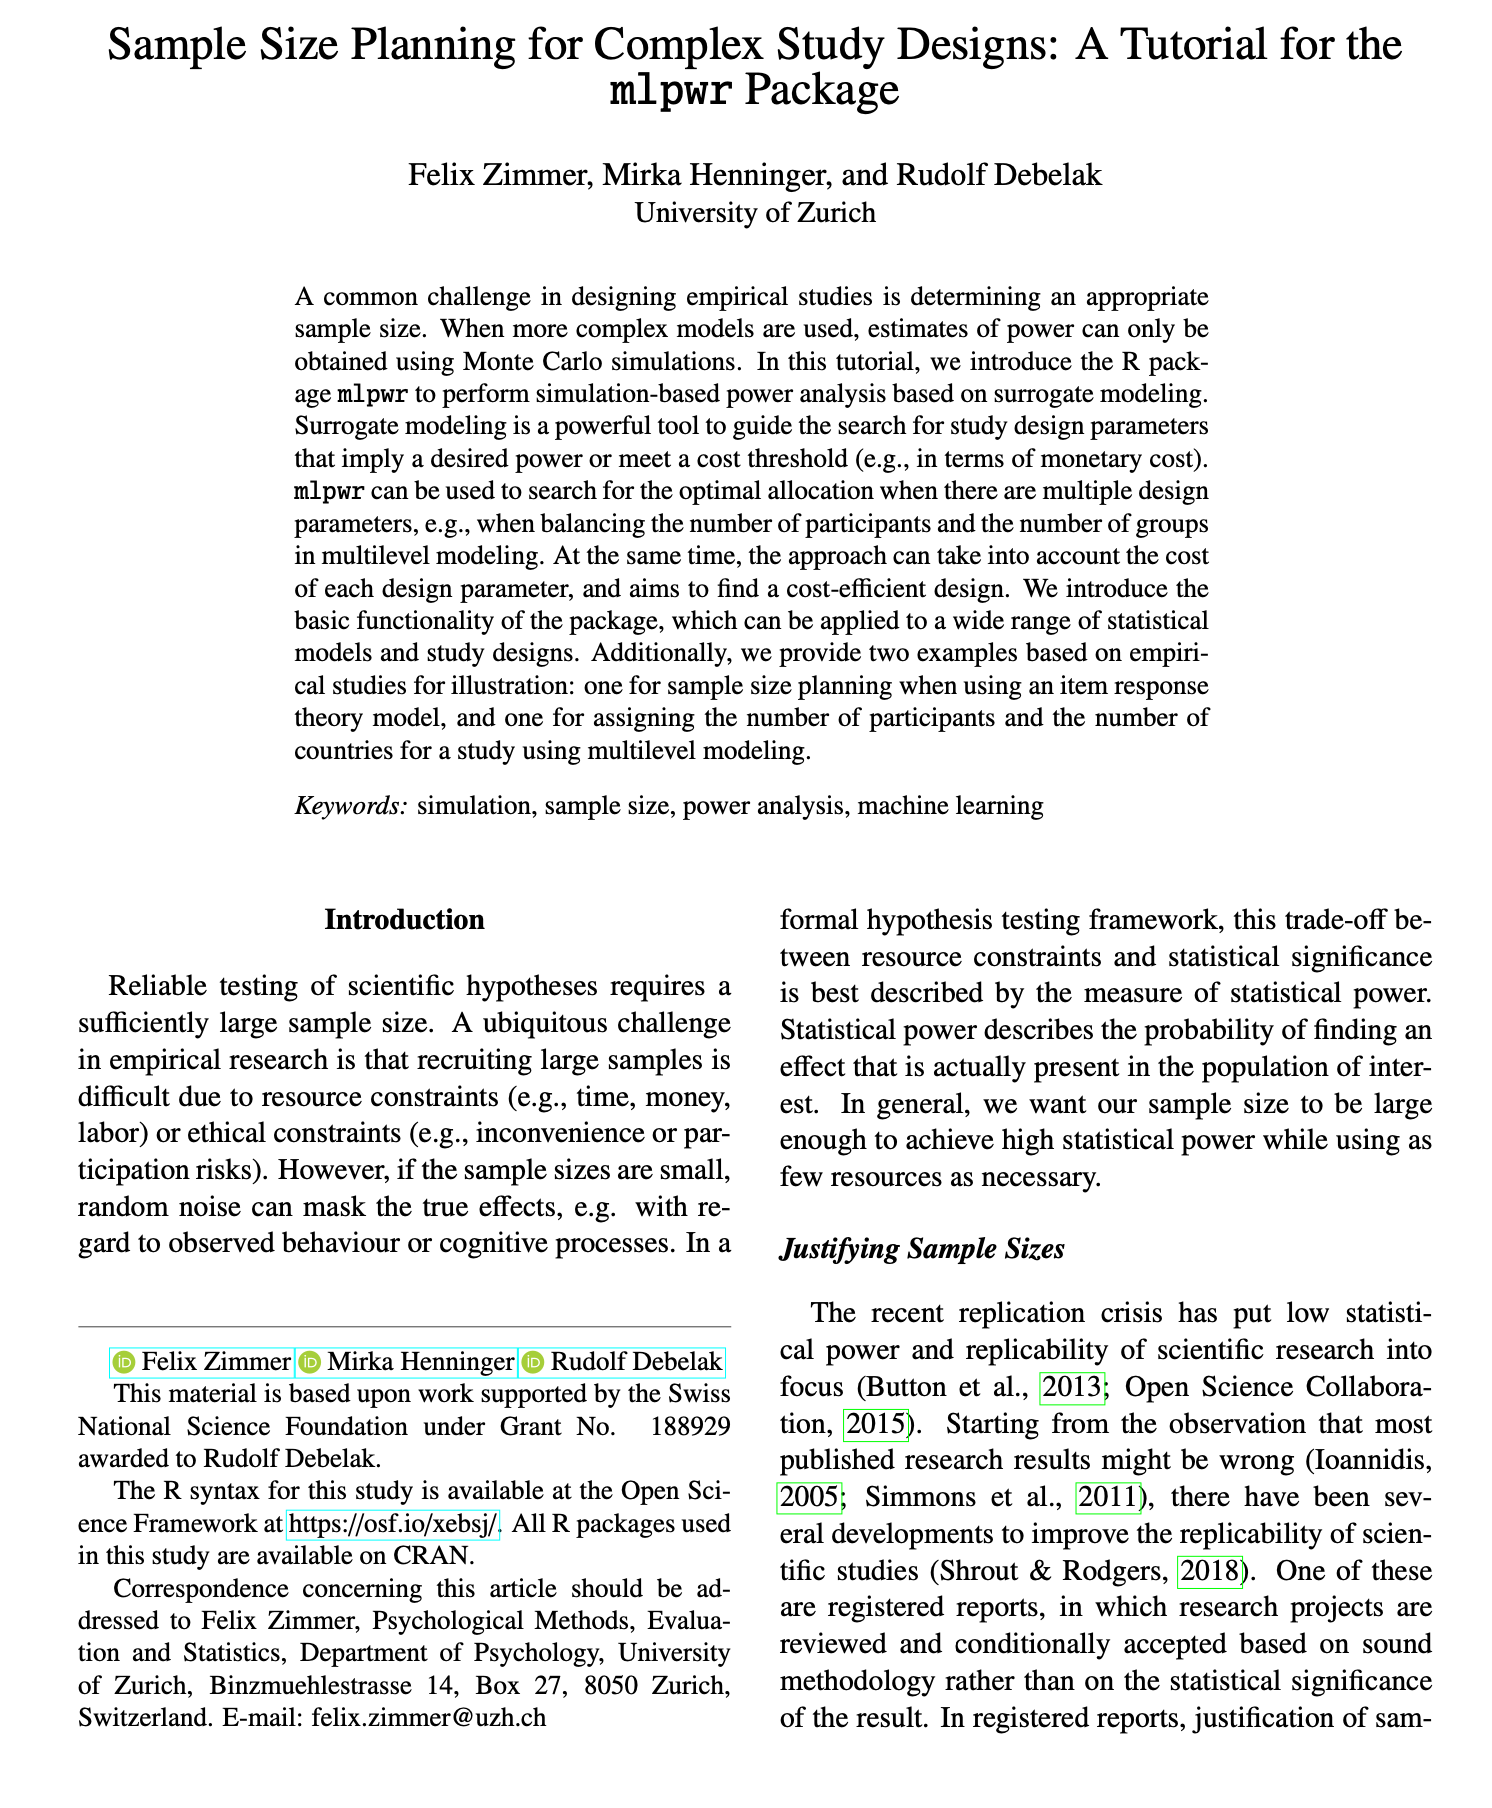
\includegraphics[width=\textwidth]{figures/mlpwr_paper.png}
		\end{column}
	\end{columns}

\end{frame}

\begin{frame}[t]{Surrogate modeling}

	\begin{itemize}
		\item Surrogate modeling aims to approximate a relationship that is
		      costly to investigate with a cheaper function (Bhosekar \&
		      Ierapetritou, 2018; Forrester \& Keane, 2009).

		\item  We can adopt the idea of surrogate modeling to the functional
		      relationship between study design parameters and power.

		\item Using this functional relationship, we can predict the power for
		      a sample size that we did not perform a simulation at
		      beforehand.

		\item Surrogate modeling is more efficient than grid search: In a
		      simple example, our approach required only 20\% of the
		      computational effort and performed 50\% more simulation runs
		      that used the optimal sample size (Zimmer \& Debelak, 2022).

	\end{itemize}

\end{frame}

\begin{frame}[c]{Example}

	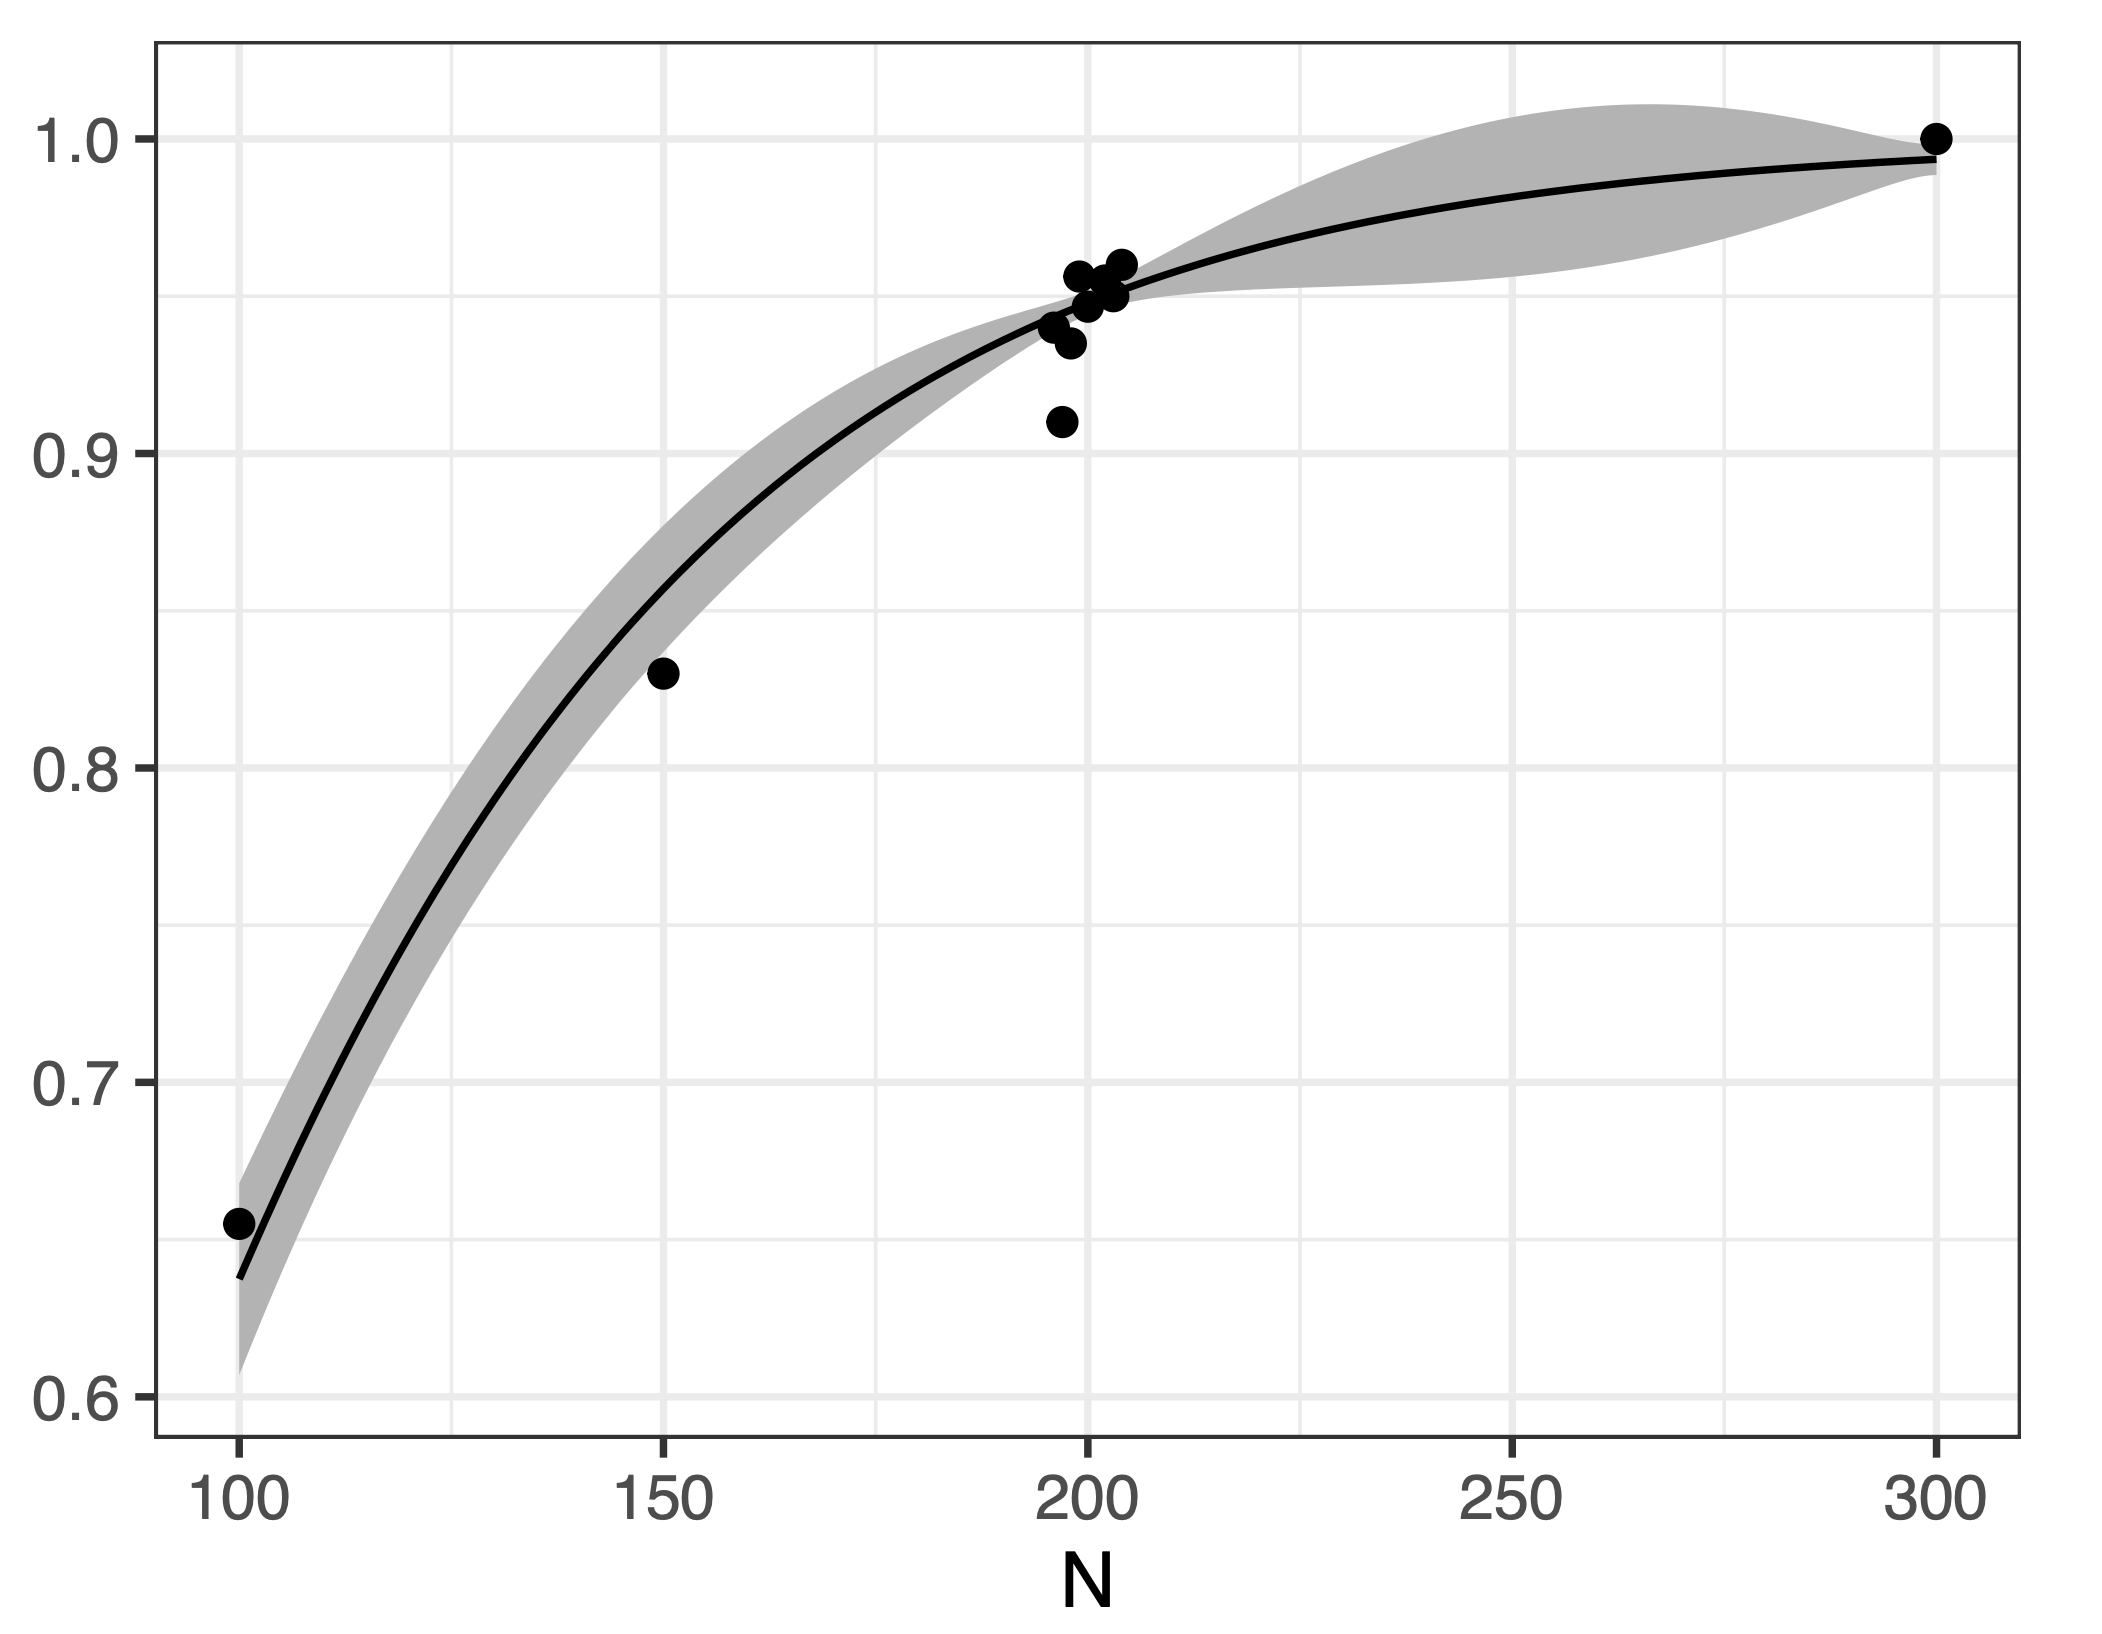
\includegraphics[width=\textwidth]{figures/mlpwr_example.png}

\end{frame}

\begin{frame}[t]{Slide explaining how we calculate the final sample size}
	\begin{enumerate}
		\item User specifies input parameters
		      \begin{cbox}{KCLtealblue}{}
			      \begin{itemize}
				      \item The expected large sample performance of the
				            model.
				      \item The range of sample sizes over which to search.
				      \item The number of signal and noise parameters.
				      \item The expected outcome prevalence.
			      \end{itemize}
		      \end{cbox}
		\item Set data, model, and metric functions based on user input
		      \begin{cbox}{KCLtealblue}{}
			      \begin{itemize}
				      \item Use defaults, but can be specified (e.g.\
				            \texttt{model = ``lasso''}).
			      \end{itemize}
		      \end{cbox}

		\item Tune the data generating model
		\item Perform search; return minimum sample meeting criteria.
	\end{enumerate}

	\sgap

\end{frame}

\begin{frame}[t]{CRITERIA}

	We then return the minimum sample that is within 10\% of expect large
	sample performance in 80\% of replications.

	If we had unlimited data, what's possible? Best case. What is the sample
	size that is sufficient to be within 10\% of this maximum achieveable.

	How many replications?

\end{frame}

\begin{frame}[t]{Example 1:\ Binary outcome, logistic regression }

	including comparison with \texttt{pmsampsize}

\end{frame}

\begin{frame}[t]{Example 2:\ Binary outcome, LASSO regression }

\end{frame}

\begin{frame}[t]{Example 3:\ Custom model function}

	\texttt{simulate\_custom}

	XGBoost

\end{frame}

\begin{frame}[t]{Maybe put slide with simulations here?}

	With our package we can replicate other criteria.

	How would it look if we included pmsampsize criteria within pmsims
	framework?

	For example, shrinkage from \texttt{pmsampsize}:

	DEMO

	We can accomodate any.
\end{frame}

\begin{frame}[t]{Development status}
	Package in development; functioning, but more testing needed.

	\begin{itemize}
		\item Follow
		      \href{https://fediscience.org/@ewan}{\textcolor{KCLseablue}{fediscience.org/@ewan}}
		      for updates.
		\item Or enter an email address at
		      \href{https://tinyurl.com/pmsims-announce}{\textcolor{KCLseablue}{tinyurl.com/is-it-ready-yet}}
		      to get one email when a public release is available.
	\end{itemize}

	Please come and talk to us.

	Criteria/models/etc. all subject to change.

\end{frame}

\begin{frame}[t]{What's next? (1/2)}

\begin{cbox}{KCLtealblue}{1.\ Machine learning}{}

\end{tcolorbox}

\begin{cbox}{KCLpurple}{2.\ Longitudinal data}{}

\end{tcolorbox}

\end{frame}

\begin{frame}[t]{What's next? (2/2)}

\begin{cbox}{KCLseablue}{3.\ Common data types}{}
e.g., clinical, NLP, genetic.

\end{tcolorbox}

\begin{cbox}{KCLhotpink}{4.\ Performance}{}

\end{tcolorbox}

\end{frame}

\section{Conclusion}

\begin{frame}
	Thank you for listening.
\end{frame}

\appendix

\begin{frame}[allowframebreaks]{References}
    \renewcommand*{\bibfont}{\scriptsize}
	\printbibliography
\end{frame}

\end{document}
